\section{Benchmark NIST-7 "Boundary Line Singularity"}
\label{sec:bench-7}

This is a singularity problem with the solution that is singular along the left part of the boundary.
The equation solved in this problem is the Poisson's equation. 

\begin{equation} \label{boundary-line-singularity}
-\Delta u = f,
\end{equation}

in the domain $\Omega = (0, 1)^2$, equipped with Dirichlet boundary conditions
given by the exact solution. The exact solution:

\begin{equation}\label{exact-nist-7}
u(x,y) = x^{\alpha},
\end{equation}

where $\alpha \geq 0.5$ determines the strength of the singularity.
The right-hand side $f$ is calculated by inserting (\ref{exact-nist-7}) into (\ref{boundary-line-singularity}).
The solution of NIST-7 with $\alpha = 0.6$ is shown in Fig. \ref{fig:sln-nist07}.

\begin{figure}[!ht]
\centering
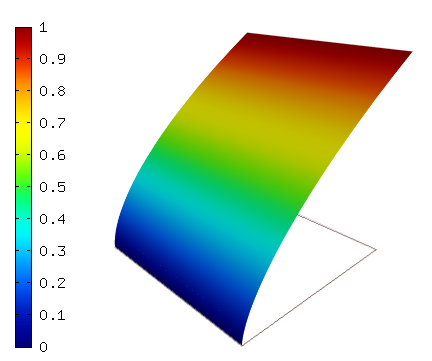
\includegraphics[height=6cm]{nist/nist-7/solution.png}
\caption{The solution to NIST-7 benchmark problem.}
\label{fig:sln-nist07}
\end{figure}

The goal of the benchmark is to reach a relative error below
$1.5$~\% in the $H^1$-norm with as few DOFs as possible.
We begin with adaptive $hp$-FEM,
the initial mesh is shown in Fig. \ref{fig:nist-7-hp-aniso} (left).
After 43 adaptivity steps, the resulting mesh with 88 DOF is shown
in Fig. \ref{fig:nist-7-hp-aniso} (right).

\begin{figure}[!ht]
\centering
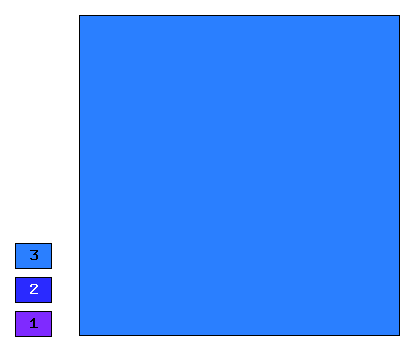
\includegraphics[height=5cm]{nist/nist-7/mesh_hp_aniso_init.png}\ \
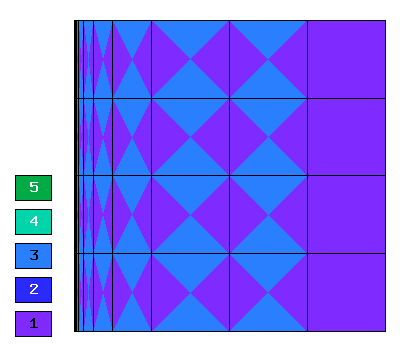
\includegraphics[height=5cm]{nist/nist-7/mesh_hp_aniso.png}
\caption{Initial mesh (left) and final mesh (right) for $hp$-FEM with anisotropic refinements.}
\label{fig:nist-7-hp-aniso}
\end{figure}

The final relative error estimate in $H^1$-norm was 1.46348 \%,
and it was identical to the exact error in all printed digits.
We also solved this benchmark with adaptive $h$-FEM
with linear (left) and quadratic (right)
elements, with anisotropic refinements enabled.
Final meshes for the $h$-FEM computations are shown
in Fig. \ref{fig:nist-7-h-aniso}.

\begin{figure}[!ht]
\centering
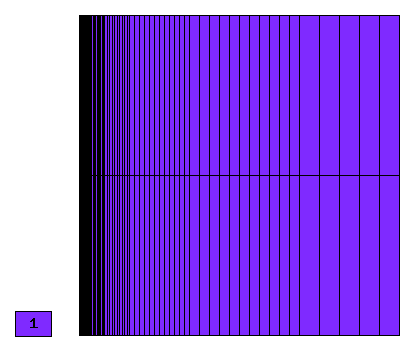
\includegraphics[height=5cm]{nist/nist-7/mesh_h1_aniso.png}\ \
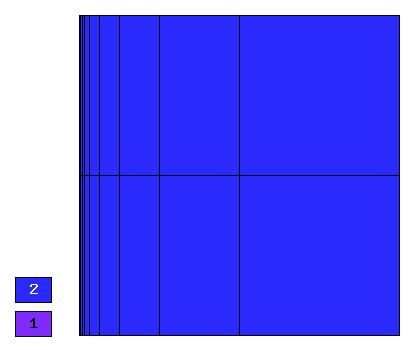
\includegraphics[height=5cm]{nist/nist-7/mesh_h2_aniso.png}
\caption{Final mesh for $h$-FEM anisotropic refinements with linear and quadratic elements.}
\label{fig:nist-7-h-aniso}
\end{figure}

Finally, Figs. \ref{fig:nist-7-conv} compare all
three approaches to automatic adaptivity from the point
of view of DOF and CPU convergence.

\begin{figure}[!ht]
\centering
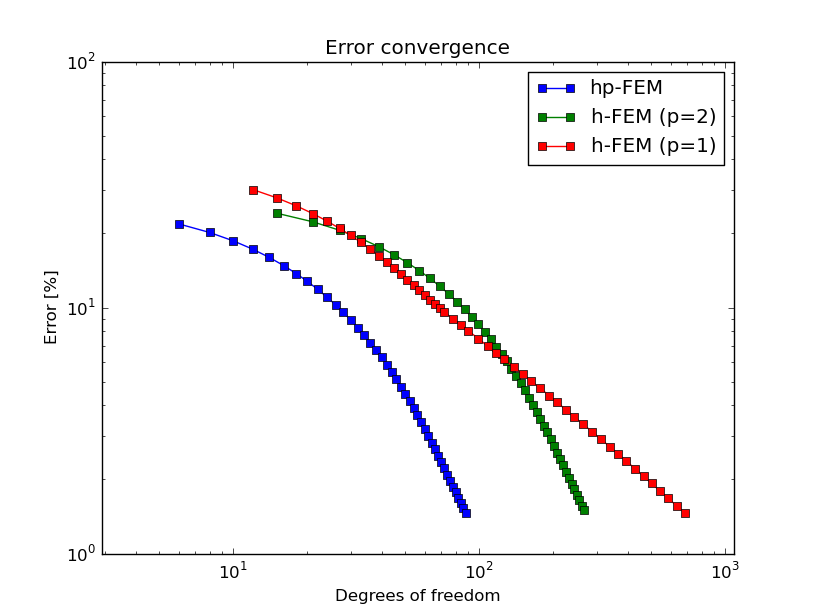
\includegraphics[height=5cm]{nist/nist-7/conv_dof_aniso.png}\ \
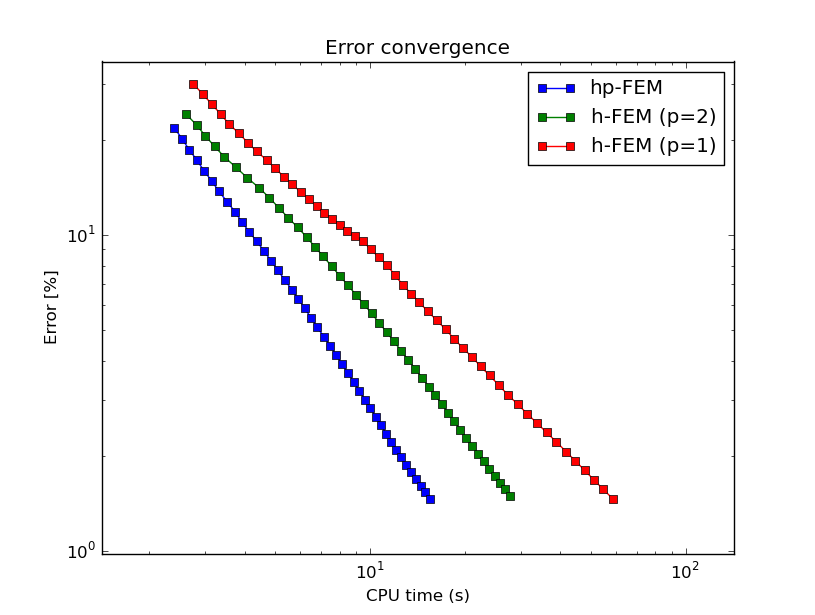
\includegraphics[height=5cm]{nist/nist-7/conv_cpu_aniso.png}
\caption{DOF and CPU time convergence graphs.}
\label{fig:nist-7-conv}
\end{figure}

